We perform the analysis on a dataset corresponding to \intlumi\ integrated luminosity. 
In this section we document the results obtained after the $\zz$ preselection defined in 
Section~\ref{sec:selection} and the final mass-dependent $\hzz$ selections using cut-based approach. 

\subsection{Results after looser selections}

We compare the data with simulation in looser selections than the signal region 
to verfity the agreement in the key kinematic observables that we select on. 

To verify the data to simulation agreement, we study the 
Figure ~\ref{fig:zpt_zzpresel} shows the dilepton $p_T$ spectrum with a 
very loose cut on the \met\ ($>20\GeVcc$), which is applied to account for the data skimming requirements. 
We select on the dilepton $p_T$ to be above 25 \GeV\  to reduce the \dyll\ contributions. 
A comparison of the predicted Z+jets \met distributions is show in Figure \ref{fig:metcomparison_zzpresel}.

Table~\ref{tab:zzselection_all} shows the number of events observed in
data, comparing to the expected background contribution at the \zz
preselection level. The background estimation was discussed at Section~\ref{sec:backgrounds}.
The $M_T$ distributions are shown in Figure \ref{fig:mt_zzpresel} after 
applying the \zz preselection. 

%%%%%%%%%%%%%%%%%%
\begin{table}[!ht]
\begin{center}
\begin{tabular}{c|c|c|c}
\hline
sample 	& mm 	& ee 	 & TOTAL\\ \hline 
WW	& 53.69 $\pm$ 2.38	& 42.35 $\pm$ 2.13	& 96.04 $\pm$ 3.19 \\
ZZ	& 36.43 $\pm$ 0.38	& 26.21 $\pm$ 0.33	& 62.64 $\pm$ 0.50 \\
WZ	& 31.22 $\pm$ 0.51	& 23.74 $\pm$ 0.45	& 54.96 $\pm$ 0.69 \\
Top	& 48.30 $\pm$ 0.70	& 34.71 $\pm$ 0.62	& 83.01 $\pm$ 0.93 \\
DYtt	& 1.68 $\pm$ 0.63	& 1.74 $\pm$ 0.65	& 3.42 $\pm$ 0.90 \\
Zjets	& 438.72 $\pm$ 12.12	& 311.74 $\pm$ 8.29	& 750.46 $\pm$ 14.69 \\
\hline
Total background	& 610.05 $\pm$ 12.40	& 440.49 $\pm$ 8.63	& 1050.54 $\pm$ 15.11 \\ \hline 
DATA	& 572 	& 478	& 1050 \\ \hline 
\end{tabular}
\caption{Expected number of signal and background events from the data-driven methods for an 
 integrated luminosity of \intlumi after applying the \zz preselections. Only statistical uncertaities are reported. 
The $\Wjets$ background is neglible thus omitted in the table.}
\label{tab:zzselection_all}
\end{center}
\end{table}
%%%%%%%%%%%%%%%%%%


%%%%%%%%
\begin{figure}[!hbtp]
\begin{center}
\label{fig:zpt_zzpresel}
\subfigure[0-Jet]{\label{subfig:zpt_0j}
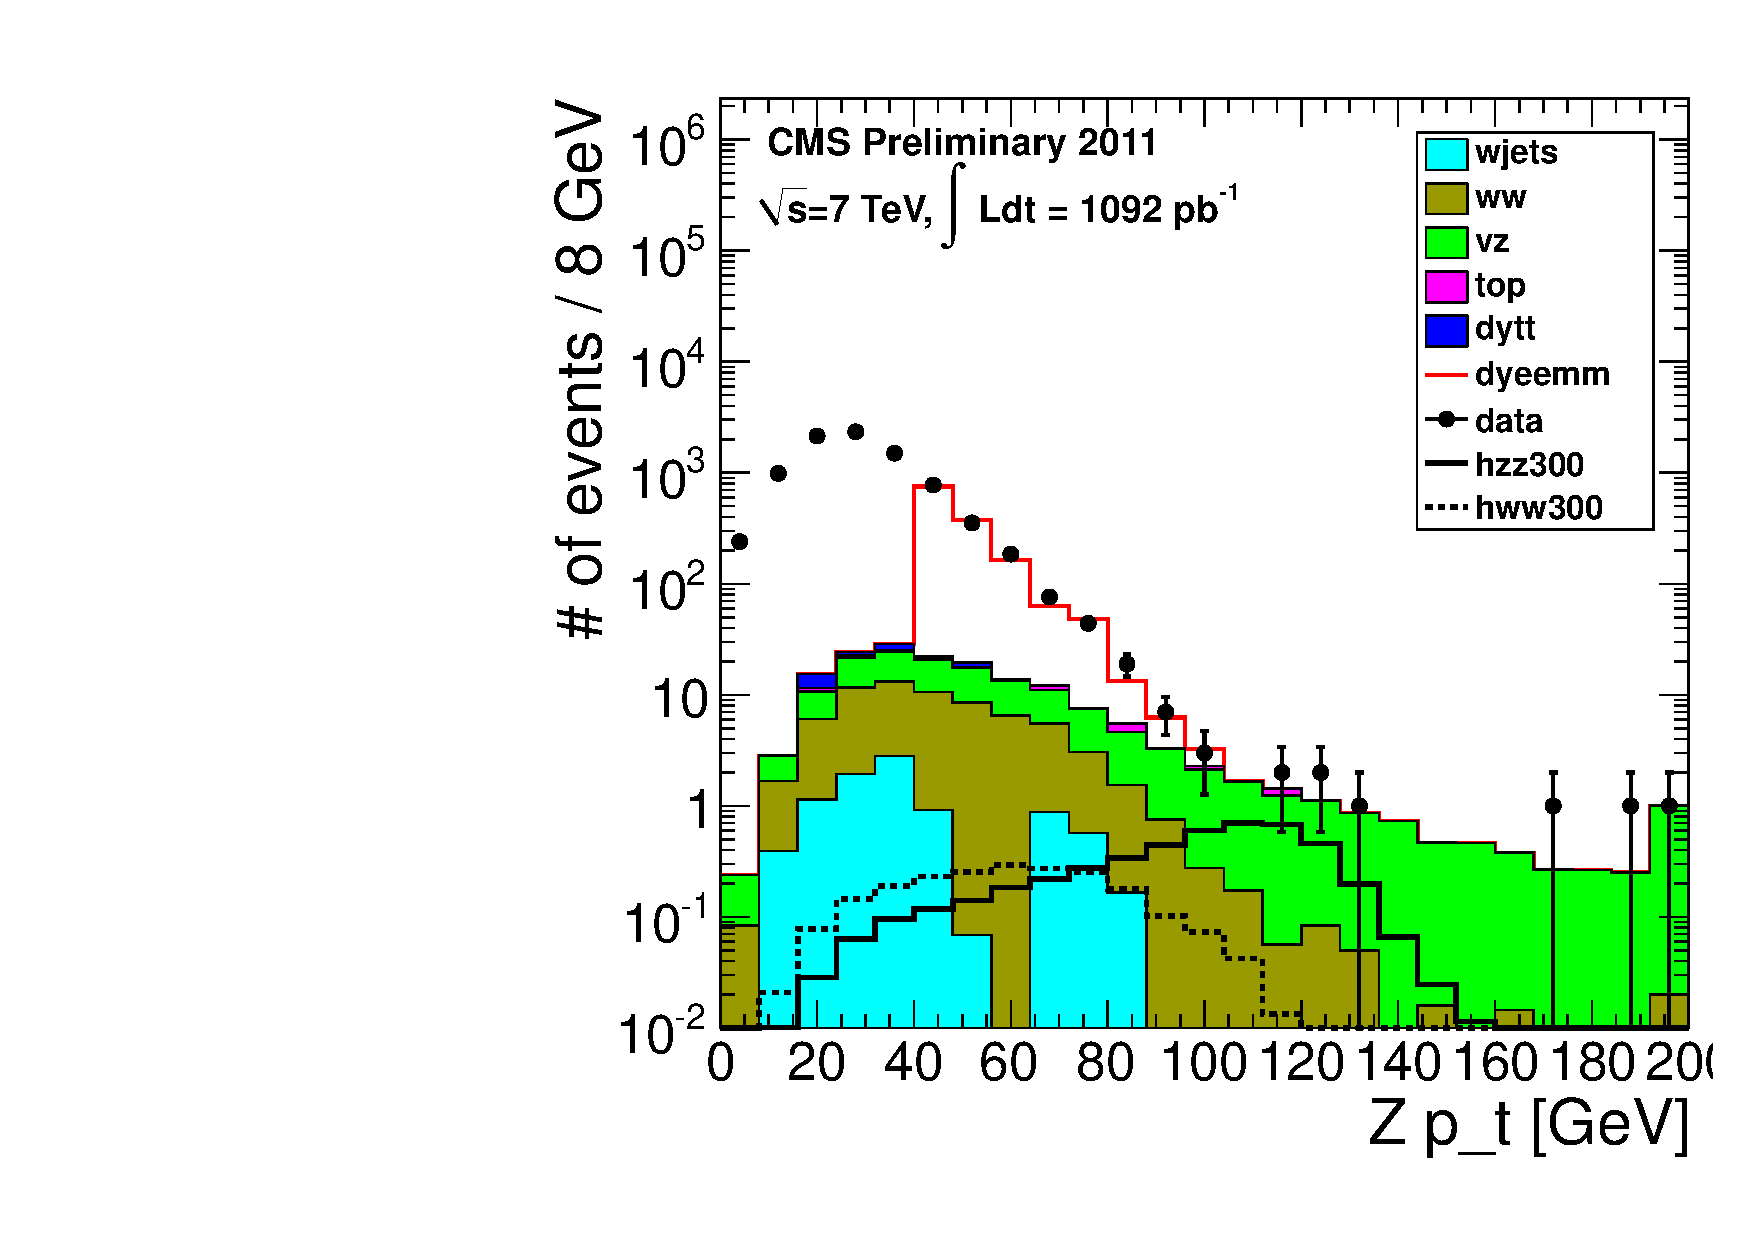
\includegraphics[width=.3\textwidth]{figures/Hm300_preselection_0jets_zpt.pdf}}
\subfigure[1-Jet]{\label{subfig:zpt_1j}
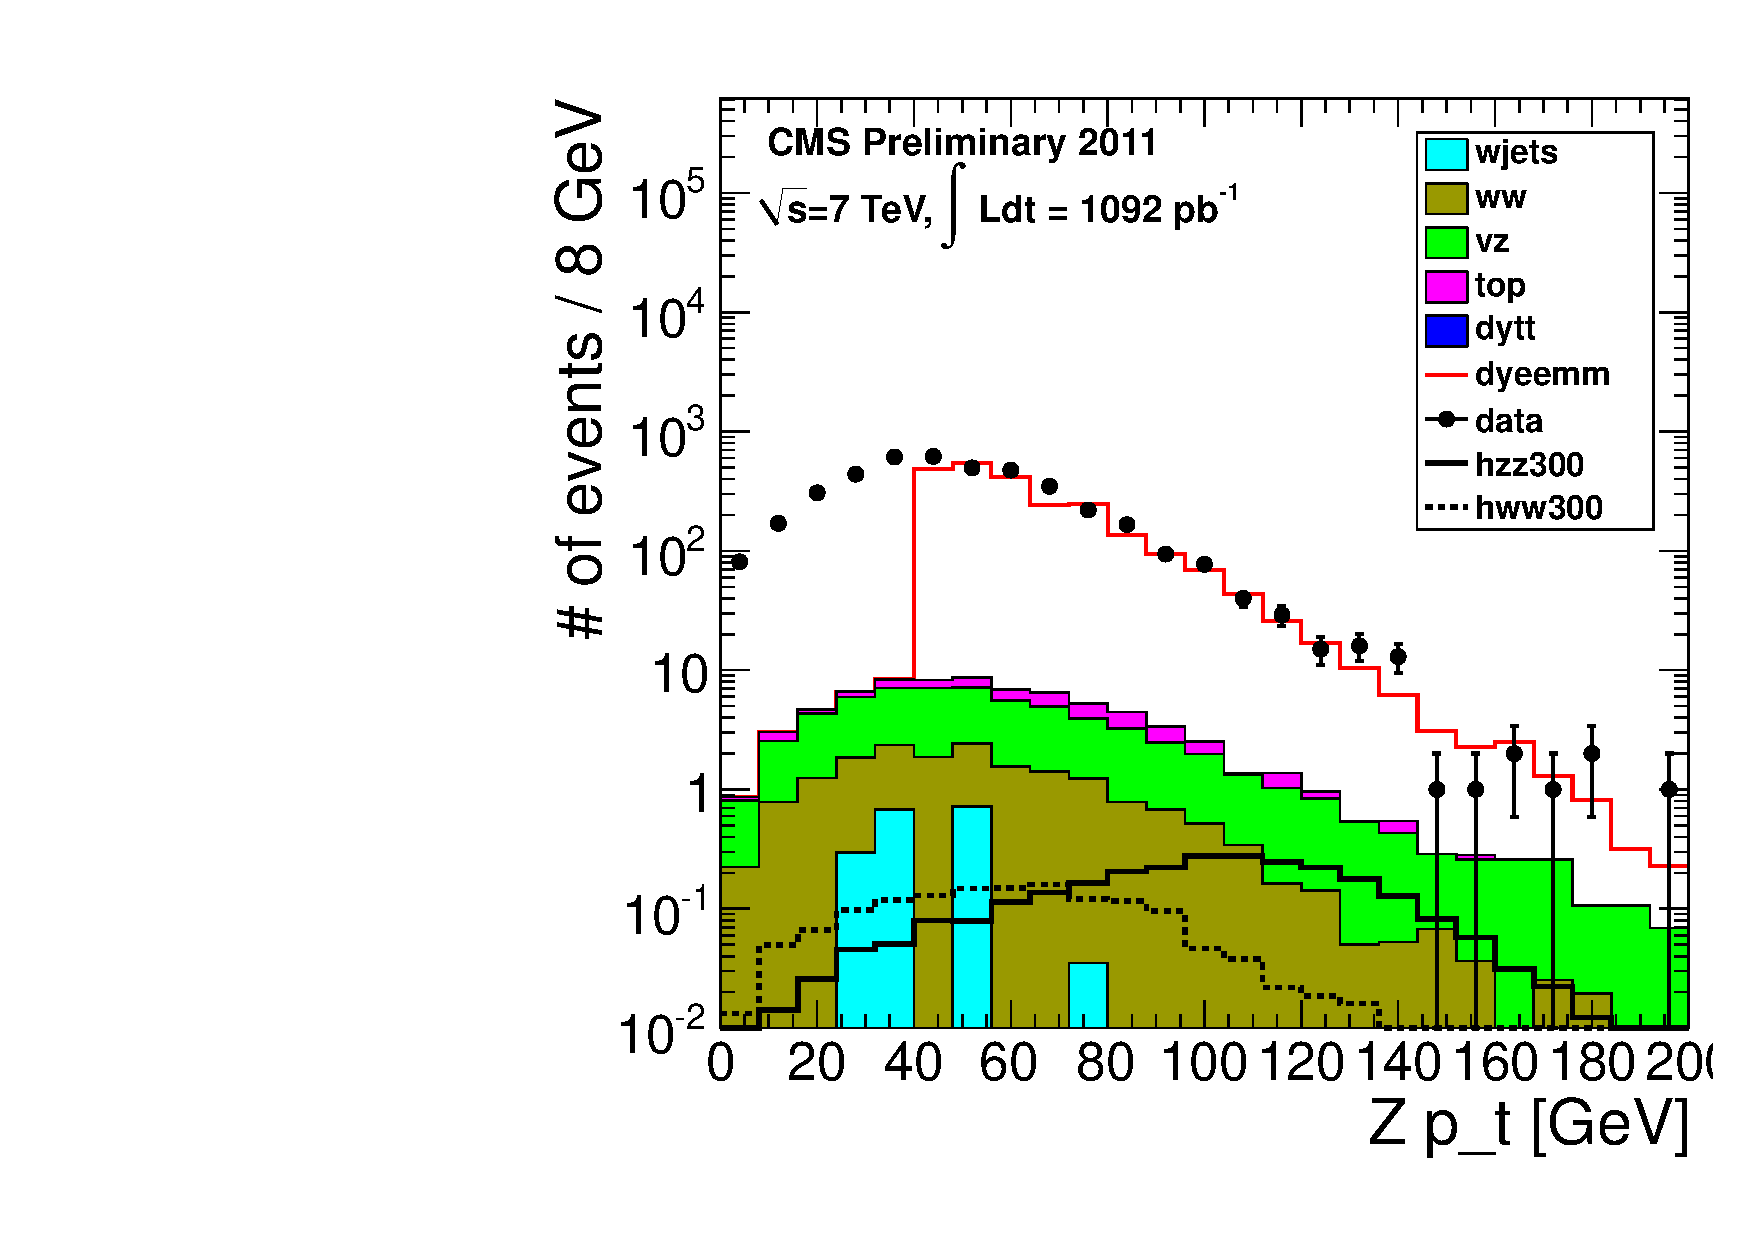
\includegraphics[width=.3\textwidth]{figures/Hm300_preselection_1jet_zpt.pdf}}
\subfigure[$\geq$2 Jets]{\label{subfig:zpt_2j}
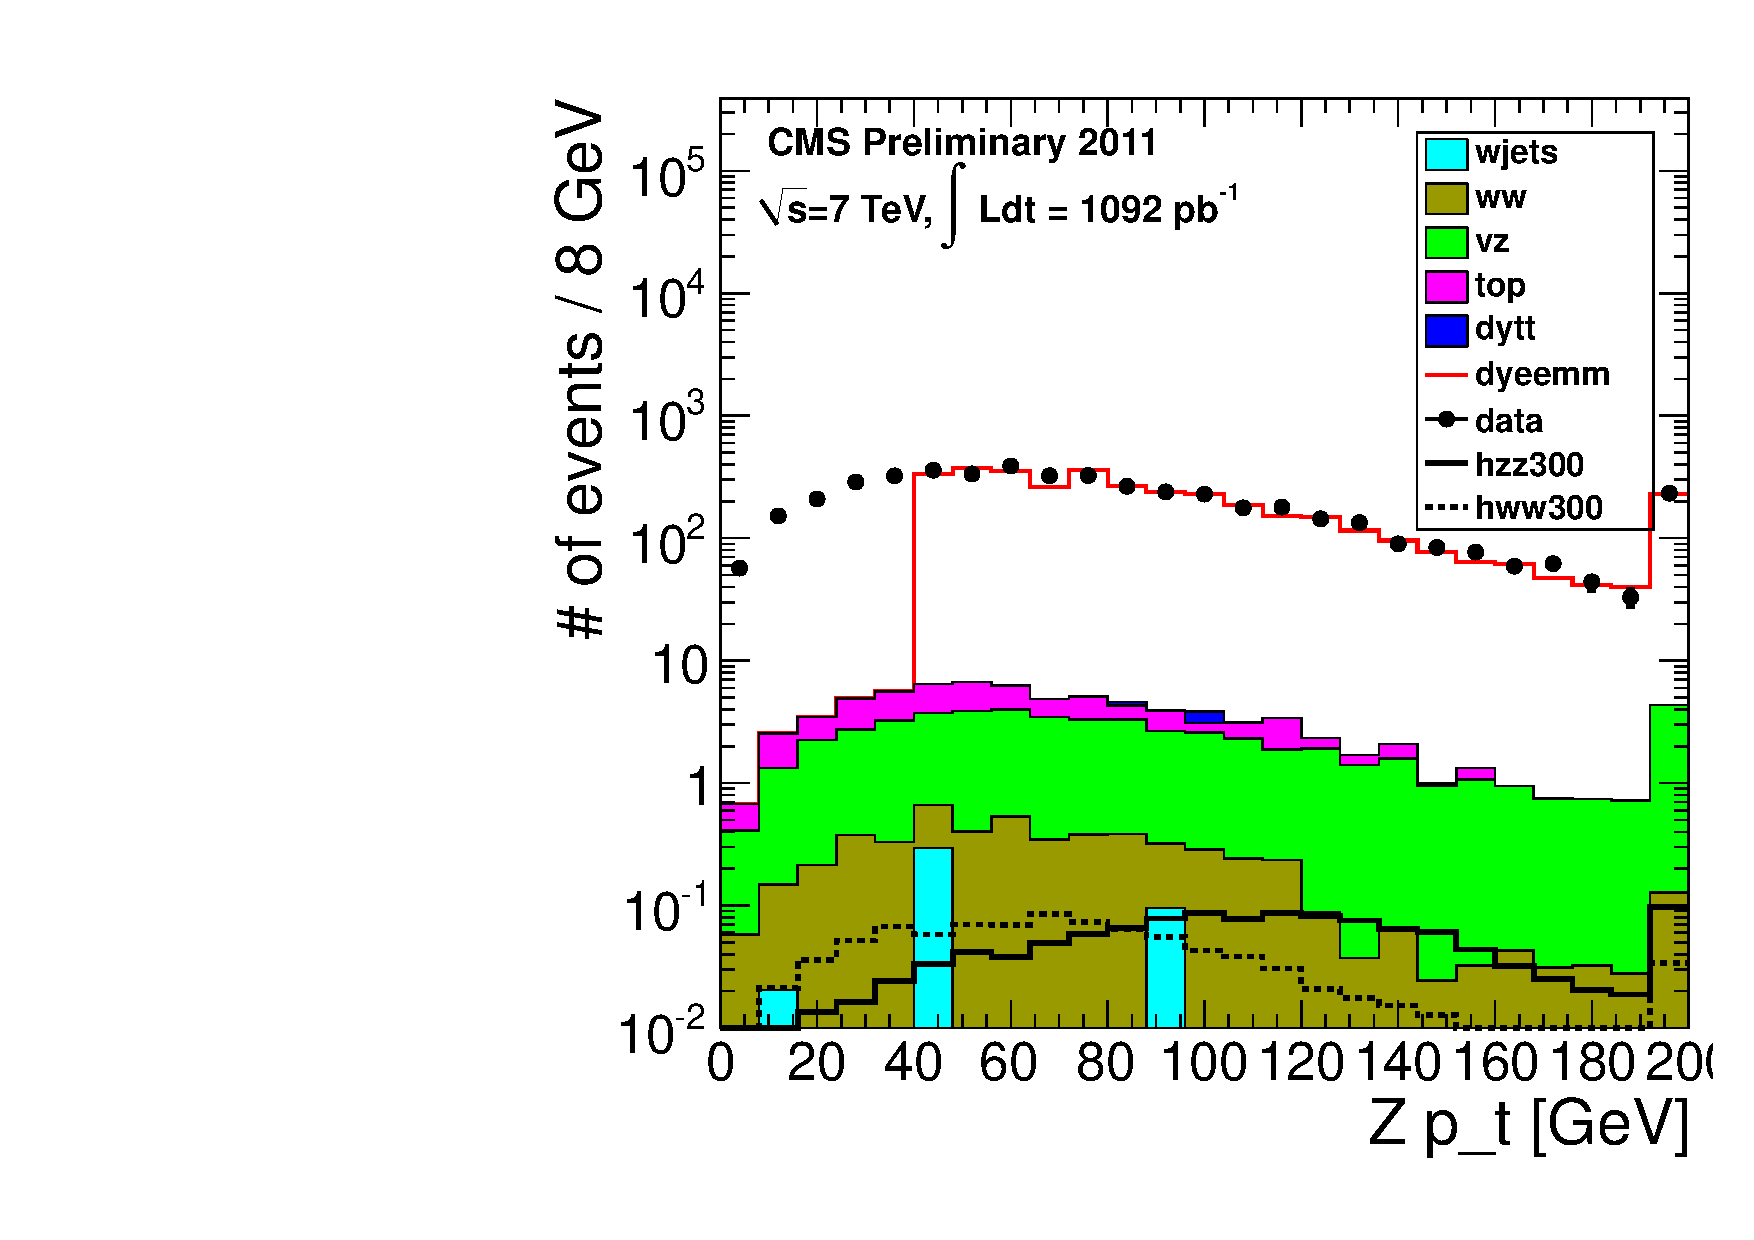
\includegraphics[width=.3\textwidth]{figures/Hm300_preselection_2jets_zpt.pdf}}
\caption{Dilepton $p_T$ distribution after the $\ZZ$ preselection observed in data corresponding to $1092\pm7$~\ipb data in 0-Jet~\subref{subfig:zpt_0j}, 1-Jet~\subref{subfig:zpt_1j}
and 2-Jet~\subref{subfig:zpt_2j} bins, compared to the expected from simulation for signal and background.
The MC backgrounds are scaled as appropriate and the photon+jets estimate of the Z+jets background is added to the stack.}
\end{center}
\end{figure}
%%%%%%%%

%%%%%%%%
\begin{figure}[!hbtp]
\begin{center}
\label{fig:metcomparison_zzpresel}
\subfigure[0-Jet]{\label{subfig:metcomparison_0j}
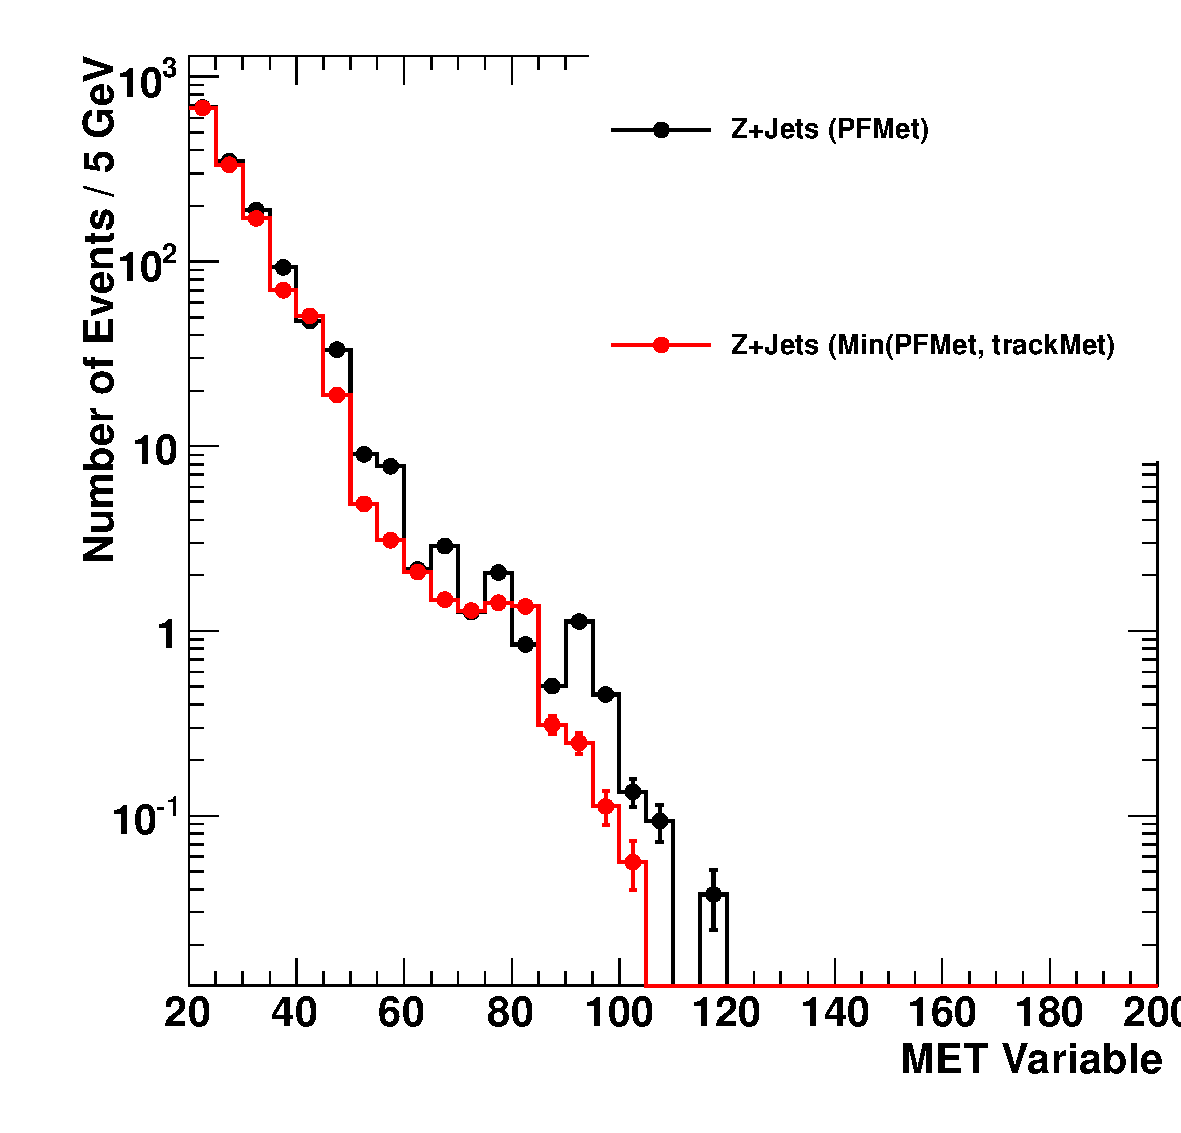
\includegraphics[width=.3\textwidth]{figures/presel_hzz300_metcomparison_0j_log.pdf}}
\subfigure[1-Jet]{\label{subfig:metcomparison_1j}
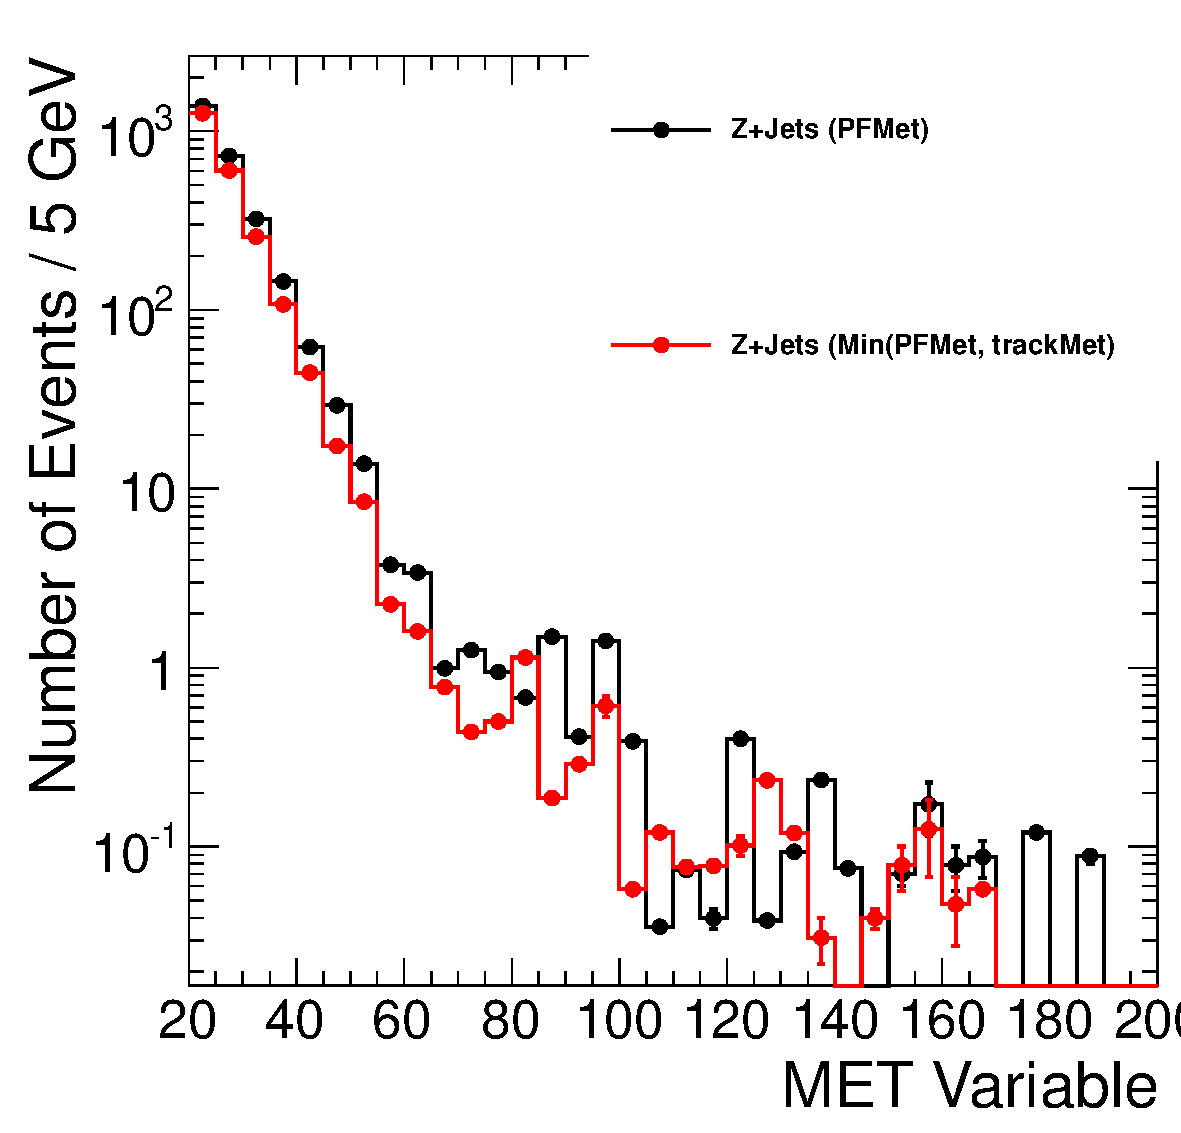
\includegraphics[width=.3\textwidth]{figures/presel_hzz300_metcomparison_1j_log.pdf}}
\subfigure[$\geq$2 Jets]{\label{subfig:metcomparison_2j}
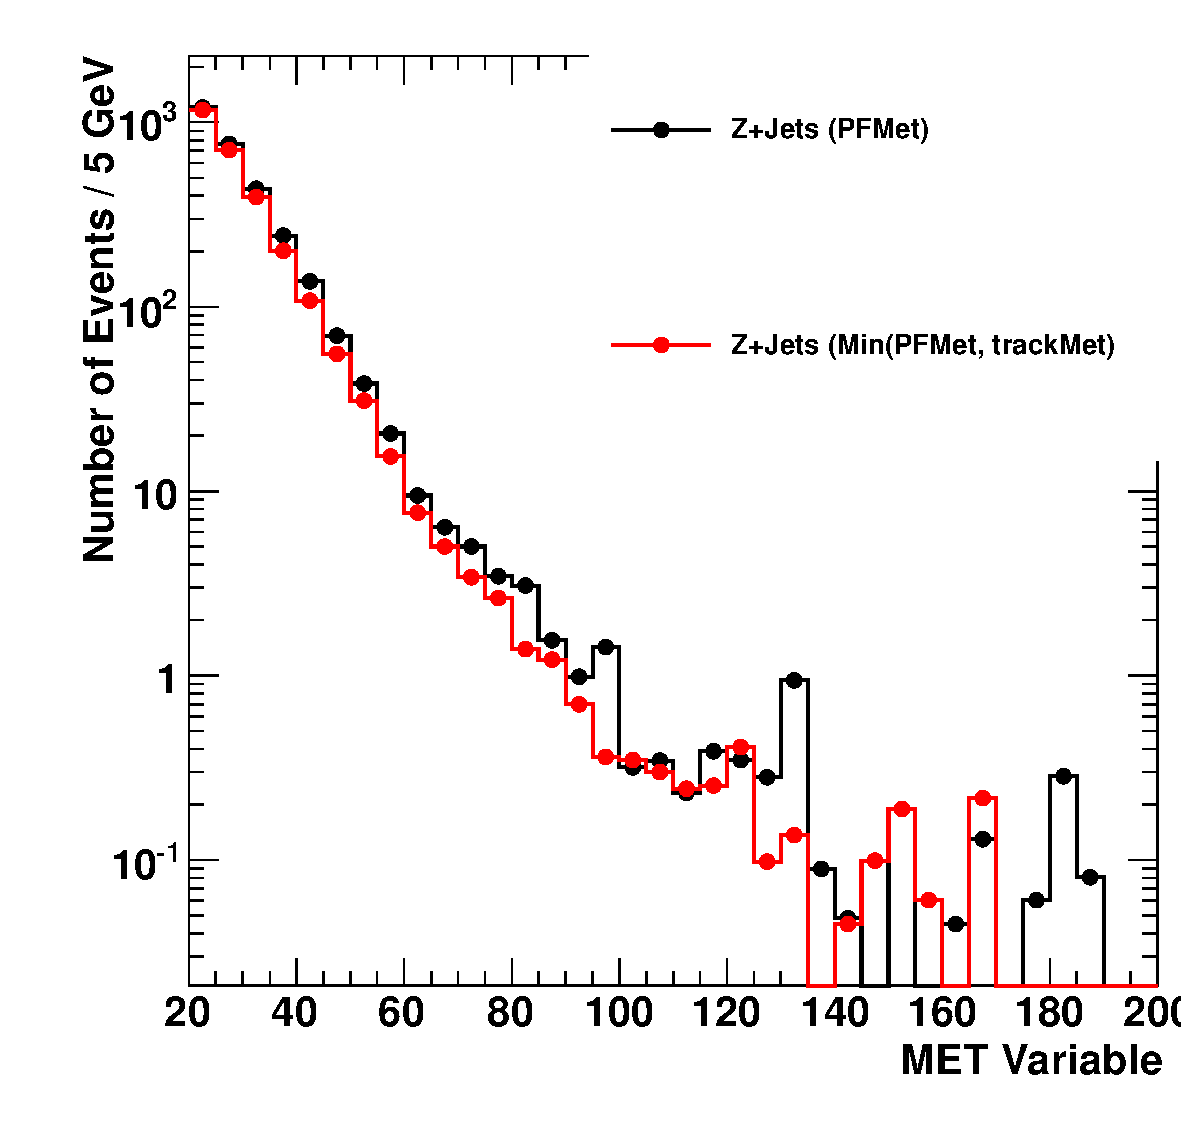
\includegraphics[width=.3\textwidth]{figures/presel_hzz300_metcomparison_2j_log.pdf}}
\caption{Comparison of the photon+jets estimate of the \met and minimum of \met and track \met distributions
after the $\ZZ$ preselection observed in data corresponding to $1092\pm7$~\ipb in 0-Jet~\subref{subfig:zpt_0j}, 1-Jet~\subref{subfig:zpt_1j}
and 2-Jet~\subref{subfig:zpt_2j} bins.}
\end{center}
\end{figure}
%%%%%%%%

%%%%%%%%
\begin{figure}[!hbtp]
\begin{center}
\label{fig:mt_zzpresel}
\subfigure[0-Jet]{\label{subfig:mt_0j}
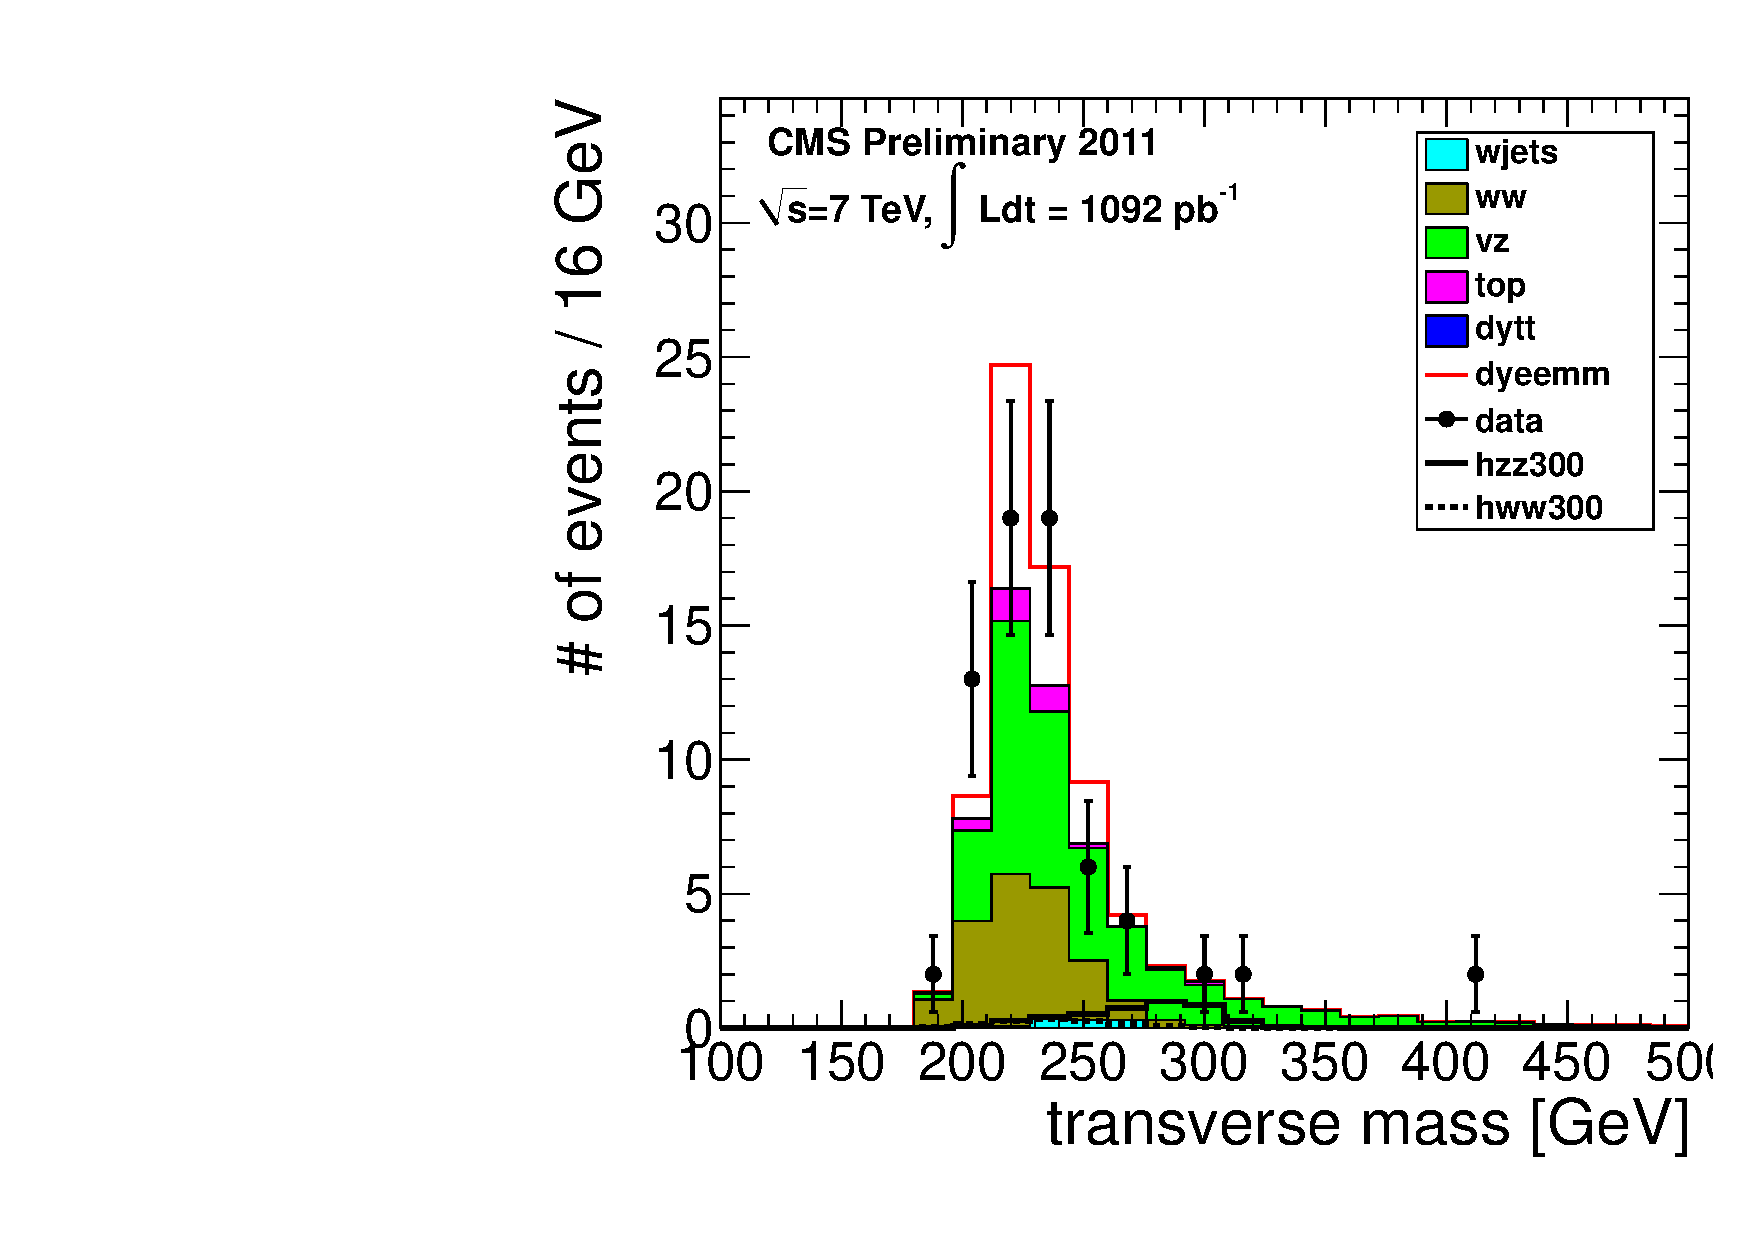
\includegraphics[width=.3\textwidth]{figures/Hm300_preselection_0jets_mt.pdf}}
\subfigure[1-Jet]{\label{subfig:mt_1j}
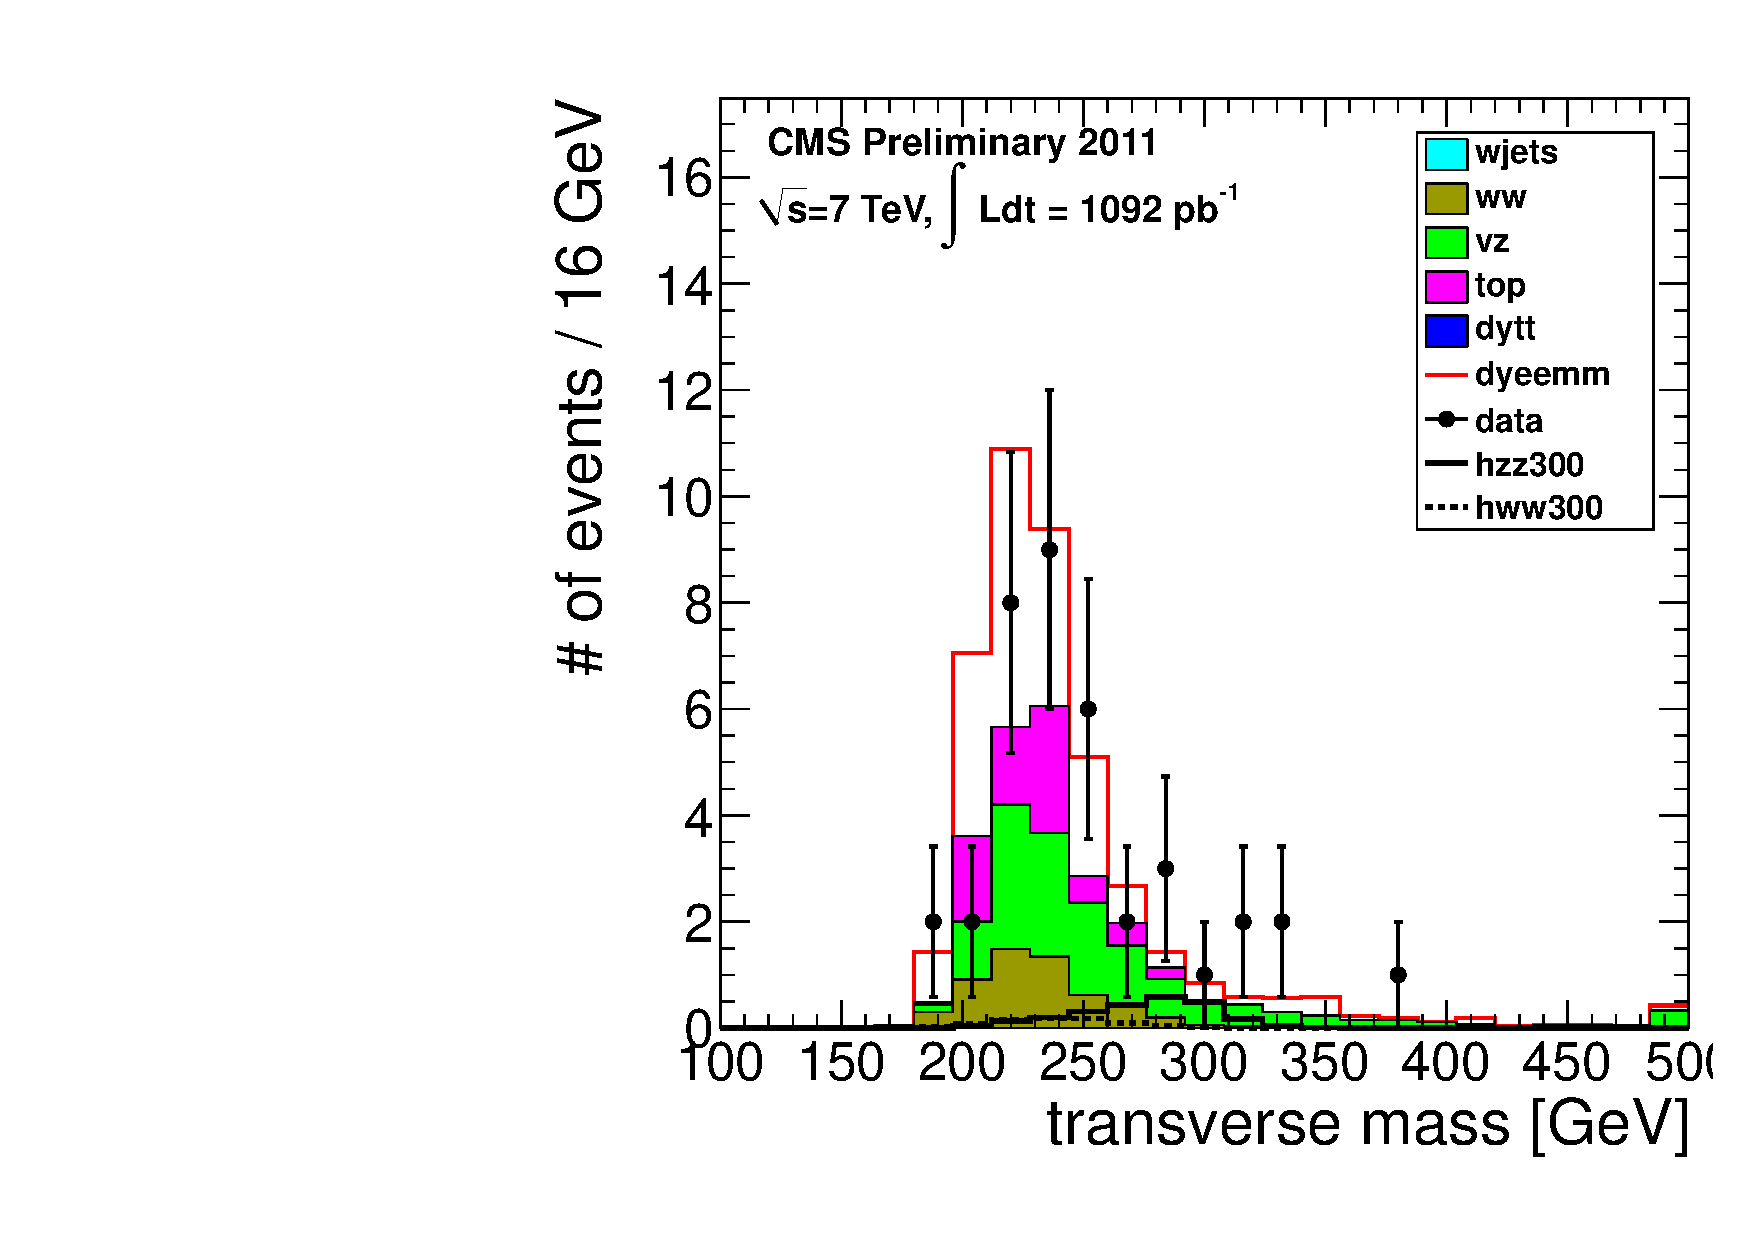
\includegraphics[width=.3\textwidth]{figures/Hm300_preselection_1jet_mt.pdf}}
\subfigure[$\geq$2 Jets]{\label{subfig:mt_2j}
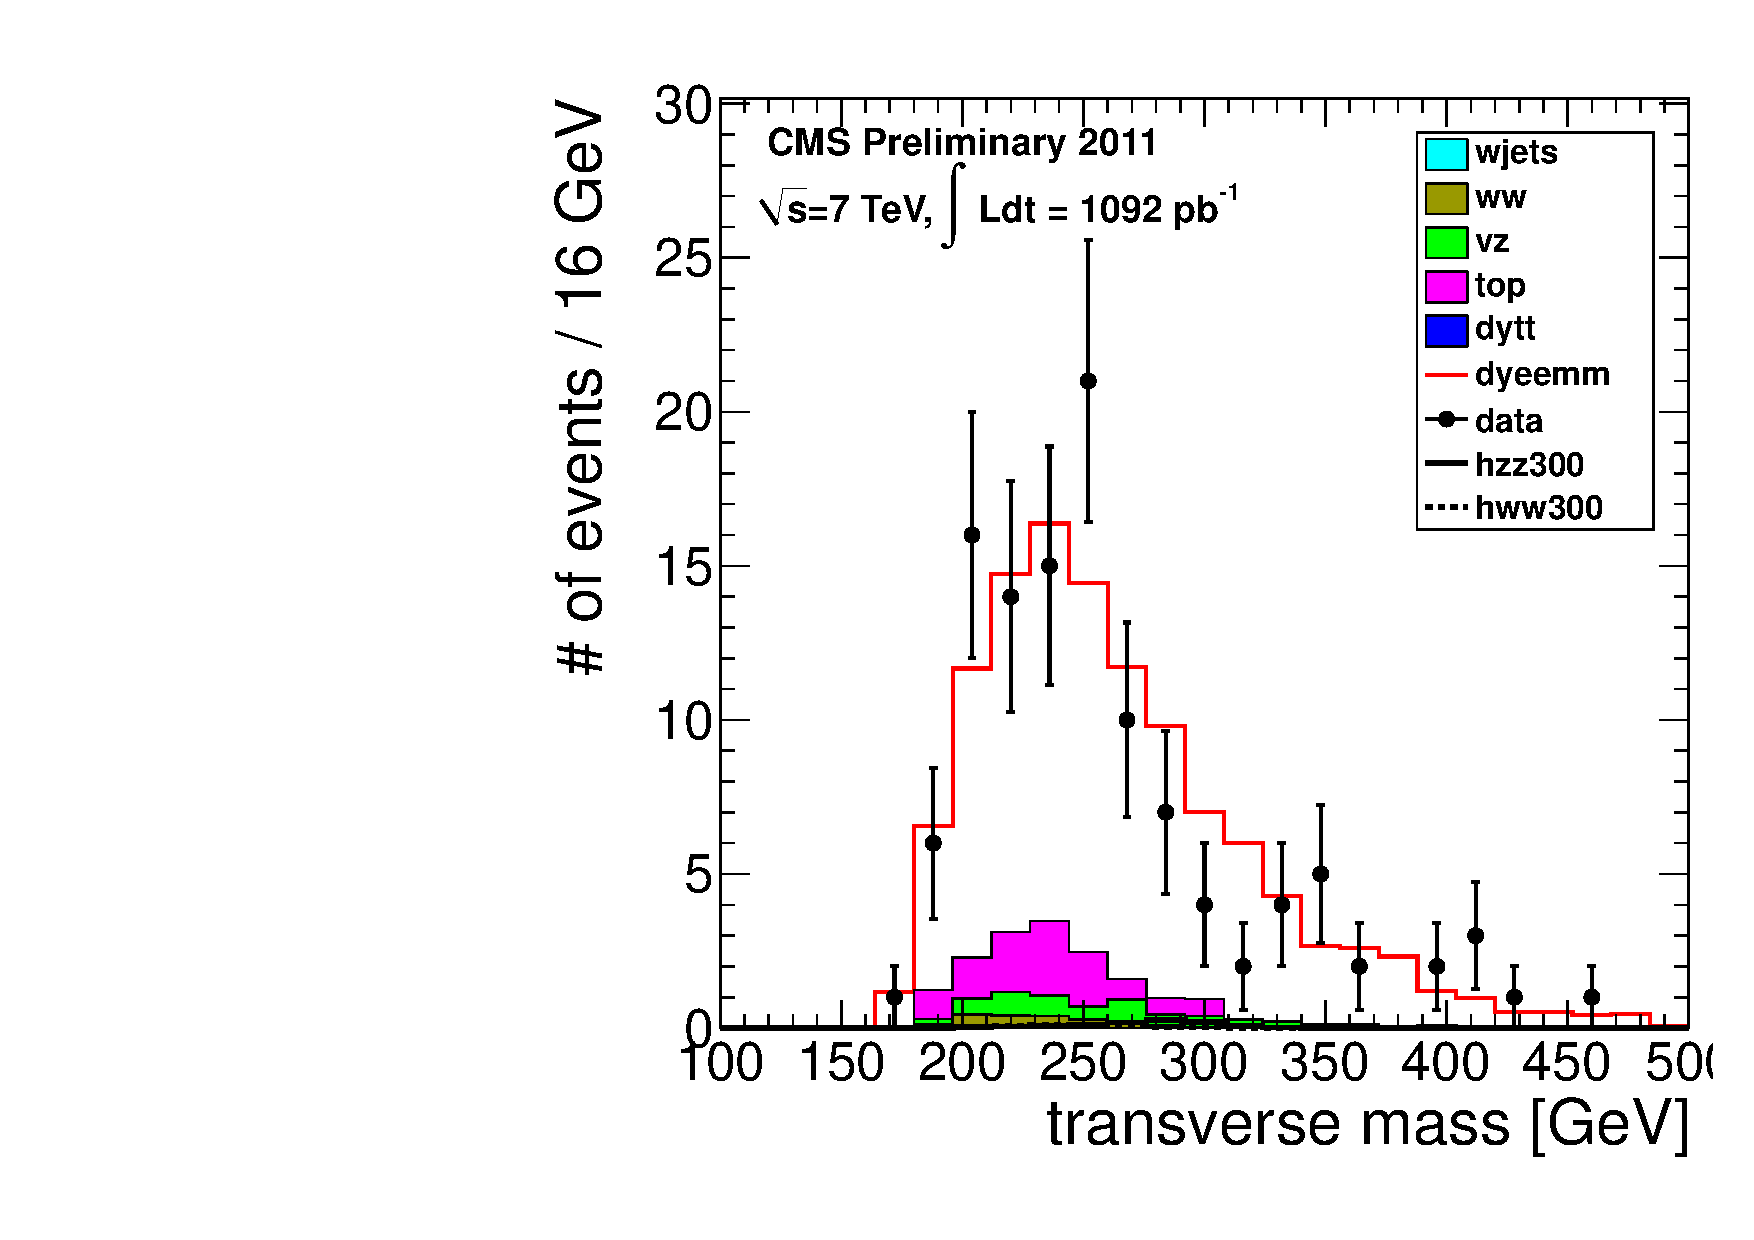
\includegraphics[width=.3\textwidth]{figures/Hm300_preselection_2jets_mt.pdf}}
\caption{Transverse mass $m_T$ distribution after the $\ZZ$ preselection observed in data corresponding to $1092\pm7$~\ipb data in 0-Jet~\subref{subfig:mt_0j}, 1-Jet~\subref{subfig:mt_1j} 
and 2-Jet~\subref{subfig:mt_2j} bins, compared to the expected from simulation for signal and background. 
The MC backgrounds are scaled as appropriate and the photon+jets estimate of the Z+jets background is added to the stack.}
\end{center}
\end{figure}
%%%%%%%%

\clearpage

\subsection{Yields after the $\hzz$ selection in cut-based analysis}

The Higgs boson mass dependent signal selections in the cut-based analysis 
are described in Section~\ref{sec:anal_cutbased}. In this section we summarise 
the results obtained all jet final states. 
Tables~\ref{tab:yield_cutbased_ee}-\ref{tab:yield_cutbased_mm} show the signal %equivalent data yields
and background expectations in ee and $\mu\mu$ final states respectively. 
As the signal region is not yet open, we tabulated the expected cross section ratio limits as a function 
of the Higgs mass, together with the 1/2-$\sigma$ uncertainty bands in Table~\ref{tab:limits_cutbased_2fb}.


%%%%%%%%%%%%%%%%%%%%%%%%%
\begin{table}
{\footnotesize
 \begin{center}
 \begin{tabular}{l | c c | c c c c c c c }
 \hline
 process & qqH & ggH & ZZ & WZ & WW & Top & Zjets & DYtt & $\sum$Bkg \\
 \hline
250 & $0.6\pm0.1$ & $5.3\pm0.8$ & $9.8\pm1.0$ & $7.6\pm0.9$ & $13.6\pm1.7$ & $12.4\pm1.0$ & $14.6\pm3.9$ & $0.0\pm0.0$ & $63.2\pm4.7$ \\ %& 48 \\
300 & $0.4\pm0.0$ & $4.1\pm0.7$ & $4.9\pm0.5$ & $3.1\pm0.4$ & $1.1\pm0.3$ & $2.5\pm0.3$ & $2.5\pm0.7$ & $0.0\pm0.0$ & $18.2\pm1.2$ \\ %& 18 \\
350 & $0.4\pm0.0$ & $4.2\pm0.7$ & $3.4\pm0.4$ & $1.7\pm0.2$ & $0.1\pm0.1$ & $0.5\pm0.1$ & $1.5\pm0.5$ & $0.0\pm0.0$ & $11.5\pm0.9$ \\ %& 10 \\
400 & $0.3\pm0.0$ & $3.7\pm0.7$ & $2.5\pm0.3$ & $1.2\pm0.2$ & $0.2\pm0.1$ & $0.1\pm0.0$ & $1.7\pm0.5$ & $0.0\pm0.0$ & $9.5\pm0.9$ \\ %& 5 \\
500 & $0.2\pm0.0$ & $1.7\pm0.4$ & $1.7\pm0.2$ & $0.6\pm0.1$ & $0.1\pm0.1$ & $0.0\pm0.0$ & $0.9\pm0.3$ & $0.0\pm0.0$ & $5.0\pm0.6$ \\ %& 3 \\
600 & $0.1\pm0.0$ & $0.6\pm0.2$ & $1.0\pm0.1$ & $0.3\pm0.1$ & $0.0\pm0.0$ & $0.0\pm0.0$ & $0.6\pm0.2$ & $0.0\pm0.0$ & $2.4\pm0.3$ \\ %& 0 \\
\hline
\end{tabular}
\end{center}
\label{tab:yield_cutbased_ee}
}
\caption{Expected number of signal and background events for an 
  integrated luminosity of \intlumi after applying the higgs selections in the cut-based analysis in the ee final state. 
  Only Monte Carlo statistical uncertainties are included. }
%\end{table}
%\begin{table}
{\footnotesize
 \begin{center}
 \begin{tabular}{l | c c |  c c c c c c c }
 \hline
 process & qqH & ggH & ZZ & WZ & WW & Top & Zjets & DYtt & $\sum$Bkg \\
 \hline
250 & $0.8\pm0.1$ & $7.2\pm1.1$ & $13.6\pm1.2$ & $10.5\pm1.1$ & $13.7\pm1.7$ & $17.4\pm1.3$ & $21.1\pm5.7$ & $0.1\pm0.1$ & $83.5\pm6.4$  \\ %& 77 \\
300 & $0.6\pm0.1$ & $5.4\pm0.8$ & $6.6\pm0.6$ & $3.6\pm0.4$ & $1.6\pm0.5$ & $3.4\pm0.3$ & $4.0\pm1.1$ & $0.0\pm0.0$ & $24.7\pm1.6$ \\ %& 17 \\
350 & $0.5\pm0.0$ & $5.5\pm0.9$ & $4.6\pm0.4$ & $2.3\pm0.3$ & $0.0\pm0.0$ & $0.8\pm0.1$ & $2.3\pm0.7$ & $0.0\pm0.0$ & $15.5\pm1.2$ \\ %& 4 \\
400 & $0.3\pm0.0$ & $4.7\pm0.8$ & $3.4\pm0.3$ & $1.5\pm0.2$ & $0.0\pm0.0$ & $0.3\pm0.1$ & $2.2\pm0.7$ & $0.0\pm0.0$ & $12.2\pm1.1$ \\ %& 7 \\
500 & $0.2\pm0.0$ & $2.1\pm0.5$ & $2.0\pm0.2$ & $0.8\pm0.1$ & $0.0\pm0.0$ & $0.0\pm0.0$ & $1.3\pm0.4$ & $0.0\pm0.0$ & $6.3\pm0.7$ \\ %& 6 \\
600 & $0.1\pm0.0$ & $0.8\pm0.3$ & $1.1\pm0.1$ & $0.4\pm0.1$ & $0.0\pm0.0$ & $0.0\pm0.0$ & $0.8\pm0.3$ & $0.0\pm0.0$ & $3.0\pm0.4$ \\ %& 2 \\
\hline
\end{tabular}
\label{tab:yield_cutbased_mm}
\end{center}
}
\caption{Expected number of signal and background events for an 
  integrated luminosity of \intlumi after applying the higgs selections in the cut-based analysis in the $\mu\mu$ final state. 
  Only Monte Carlo statistical uncertainties are included. }
\end{table}
%%%%%%%%%%%%%%%%%%%%%%%%%

\begin{table}
\begin{center}
\begin{tabular}{ccccc}
\hline
 Mass & Median Expected & [-$\sigma$, +$\sigma$] & [-2$\sigma$, +2$\sigma$]\\\hline
 250 & 1.81 & [1.25, 2.61] & [0.90, 3.65] \\
300 & 1.12 & [0.79, 1.62] & [0.58, 2.24] \\
350 & 0.73 & [0.52, 1.06] & [0.38, 1.48] \\
400 & 0.90 & [0.63, 1.32] & [0.45, 1.85] \\
500 & 1.36 & [0.95, 1.97] & [0.70, 2.78] \\
600 & 2.51 & [1.77, 3.58] & [1.33, 5.14] \\
\hline
\end{tabular}
\end{center}
\label{tab:limits_cutbased_2fb}
\caption{\fixme The median expected cross section ratio limits as a function 
of the Higgs mass, together with the 1/2-$\sigma$ uncertainty bands obtained in the cut-and-count analysis, corresponding to 
an integrated luminosity of \intlumi}
\end{table}

\subsection{Results in shape analysis} 

The Higgs boson mass dependent signal selections are described in Section~\ref{sec:signal_selection}. 
In this section we summarise the results obtained all jet final states. 
%After applying these signal selections, which differ only from the \zz preselection
%in terms of the \met and $M_T$ cuts, 
Tables~\ref{tab:yield_shapebased_ee}-\ref{tab:yield_shapebased_mm} show the signal %equivalent data yields
and background expectations in ee and $\mu\mu$ final states respectively. 
As the signal region is not yet open, we tabulated the expected cross section ratio limits as a function 
of the Higgs mass, together with the 1/2-$\sigma$ uncertainty bands in Table~\ref{tab:limits_cutbased_2fb}.


%%%%%%%%%%%%%%%%%%%%%%%%%
\begin{table}
{\footnotesize
 \begin{center}
 \begin{tabular}{l | c c | c c c c c c c }
 \hline
 process & qqH & ggH & ZZ & WZ & WW & Top & Zjets & DYtt & $\sum$Bkg \\
 \hline
250 & $0.5\pm0.1$ & $4.6\pm0.7$ & $10.3\pm1.0$ & $7.2\pm0.8$ & $9.4\pm0.9$ & $11.9\pm0.8$ & $11.3\pm2.8$ & $0.0\pm0.0$ & $54.8\pm3.4$ \\ % & 41 \\
300 & $0.6\pm0.1$ & $5.5\pm0.9$ & $12.5\pm1.2$ & $8.3\pm1.0$ & $9.5\pm0.9$ & $12.3\pm0.9$ & $11.5\pm2.9$ & $0.0\pm0.0$ & $59.7\pm3.6$ \\% & 47 \\
350 & $0.5\pm0.1$ & $5.6\pm0.9$ & $10.8\pm1.1$ & $6.4\pm0.8$ & $5.4\pm0.5$ & $10.0\pm0.7$ & $8.2\pm2.1$ & $0.0\pm0.0$ & $46.4\pm2.8$ \\% & 42 \\
400 & $0.3\pm0.0$ & $4.6\pm0.8$ & $8.2\pm0.8$ & $4.2\pm0.5$ & $1.7\pm0.2$ & $3.8\pm0.3$ & $4.8\pm1.2$ & $0.0\pm0.0$ & $27.3\pm1.8$ \\ %& 25 \\
500 & $0.2\pm0.0$ & $2.0\pm0.5$ & $7.3\pm0.7$ & $3.4\pm0.4$ & $1.1\pm0.1$ & $3.1\pm0.2$ & $3.7\pm0.9$ & $0.0\pm0.0$ & $20.7\pm1.4$ \\%& 24 \\
600 & $0.1\pm0.0$ & $0.8\pm0.3$ & $5.0\pm0.5$ & $1.9\pm0.2$ & $0.4\pm0.0$ & $1.5\pm0.1$ & $2.8\pm0.7$ & $0.0\pm0.0$ & $12.3\pm0.9$ \\% & 13 \\
\hline
\end{tabular}
\end{center}
\label{tab:yield_shapebased_ee}
}
\caption{Expected number of signal and background events for an 
  integrated luminosity of \intlumi after applying the higgs selections in the shape-based analysis in the ee final state. 
  Only Monte Carlo statistical uncertainties are included. }
%\end{table}
%\begin{table}
{\footnotesize
 \begin{center}
 \begin{tabular}{l | c c |  c c c c c c c }
 \hline
 process & qqH & ggH & ZZ & WZ & WW & Top & Zjets & DYtt & $\sum$Bkg \\
 \hline
250 & $0.7\pm0.1$ & $6.2\pm0.9$ & $14.3\pm1.2$ & $9.8\pm1.0$ & $11.1\pm1.0$ & $16.8\pm1.2$ & $15.8\pm4.0$ & $0.0\pm0.0$ & $74.1\pm4.7$ \\ % & 57 \\
300 & $0.8\pm0.1$ & $7.5\pm1.2$ & $17.4\pm1.5$ & $11.2\pm1.2$ & $11.1\pm1.0$ & $17.5\pm1.2$ & $17.1\pm4.3$ & $0.0\pm0.0$ & $81.8\pm5.1$ \\ %& 60 \\
350 & $0.6\pm0.1$ & $7.5\pm1.2$ & $14.7\pm1.3$ & $8.7\pm0.9$ & $7.0\pm0.7$ & $13.7\pm1.0$ & $12.9\pm3.2$ & $0.0\pm0.0$ & $64.7\pm4.0$ \\ %&  45 \\
400 & $0.4\pm0.1$ & $6.1\pm1.1$ & $11.3\pm1.0$ & $5.5\pm0.6$ & $1.9\pm0.2$ & $5.0\pm0.4$ & $6.2\pm1.5$ & $0.0\pm0.0$ & $36.0\pm2.2$ \\ %& 25 \\
500 & $0.2\pm0.0$ & $2.6\pm0.6$ & $9.8\pm0.8$ & $4.3\pm0.5$ & $1.1\pm0.1$ & $4.0\pm0.3$ & $5.5\pm1.4$ & $0.0\pm0.0$ & $27.3\pm1.8$ \\ %& 20 \\
600 & $0.1\pm0.0$ & $1.0\pm0.4$ & $6.5\pm0.6$ & $2.4\pm0.3$ & $0.1\pm0.0$ & $2.2\pm0.2$ & $4.0\pm1.0$ & $0.0\pm0.0$ & $16.2\pm1.2$ \\ %& 13 \\
\hline
\end{tabular}
\end{center}
}
\caption{Expected number of signal and background events for an 
  integrated luminosity of \intlumi after applying the higgs selections in the shape-based analysis in the $\mu\mu$ final state. 
  Only Monte Carlo statistical uncertainties are included. }
\label{tab:yield_shapebased_mm}
\end{table}
%%%%%%%%%%%%%%%%%%%%%%%%%

\begin{table}
\begin{center}
\begin{tabular}{ccccc}
\hline
 Mass & Median Expected & [-$\sigma$, +$\sigma$] & [-2$\sigma$, +2$\sigma$]\\\hline
 250 & 1.81 & [1.25, 2.61] & [0.90, 3.65] \\
300 & 1.12 & [0.79, 1.62] & [0.58, 2.24] \\
350 & 0.73 & [0.52, 1.06] & [0.38, 1.48] \\
400 & 0.90 & [0.63, 1.32] & [0.45, 1.85] \\
500 & 1.36 & [0.95, 1.97] & [0.70, 2.78] \\
600 & 2.51 & [1.77, 3.58] & [1.33, 5.14] \\
\hline
\end{tabular}
\end{center}
\label{tab:limits_mtshape_2fb}
\caption{\fixme The median expected cross section ratio limits as a function 
of the Higgs mass, together with the 1/2-$\sigma$ uncertainty bands obtained in the shape analysis based on $M_T$, corresponding to 
an integrated luminosity of \intlumi}
\end{table}
